\chapter{Evaluation}
\label{ch:evaluation}

This chapter discusses three different experiments that were conducted to check for effectiveness and efficiency of RDF-Doctor.
The first experiment checks the effectiveness of RDF-Doctor against set of test cases provided in~\cite{TurtleTests:Online}.
In the second experiment, a random number of errors is generated using a Poisson Distribution for a period of 8 time instances while a Uniform Distribution randomly selects types of errors for each time instance, sequentially.
%number generators for a period of time of 8 time instances to simulate a couple of syntax errors, produced by an ontology user, 
Finally, the efficiency of RDF-Doctor is measured when both, the number of errors and the size of ontologies are changed. 

In the following sections, three experiments designed to evaluate RDF-Doctor are presented. 
Each section describes a particular experiment by giving its objective, presenting the followed procedure, and discussing the achieved results.

\section{Experiment Configuration}

All experiments are run on a Linux Ubuntu 18.04 machine with a 4th Gen Intel Core i5-4300U CPU, 3MB Cache, 2.90GHz with 8GB RAM 1333MHz DDR3. 
RDF-Doctor is implemented using Java version 9. 
ANTLR framework version 4.7.1 is used to build the internal parser in RDF-Doctor.%, as well, as an imported library for compiling and running of it.  

\section{Experiment I} 
In this experiment, RDF-Doctor was validated against RDF Suite Test, specifically Turtle serialization. 
%Next text discusses the objective, shows the procedure, and finally, presents and discusses the result.  

\subsection{Objective}

There exists a number of Test Suites for each RDF serialization which is recommended by W3 Consortium (W3C) in ~\cite{TurtleTests:Online}.
%The evaluation phase starts with where a Test Suite defined in the Turtle serialization. 
These Test Suites can be used to check for the proficiency of a parser with respect to a certain serialization.% can be validated with these files found in a corresponding Test Suite. 
Therefore, the target of this experiment is to measure the proficiency of RDF-Doctor while testing with the W3C Turtle Test Suite.

\subsection{Procedure}

\begin{table}[]
\centering
\begin{tabular}{|l|c|c|c|}
\hline
 \multicolumn{1}{|c|}{\textbf{File Content}}  &{\textbf{Detected}}  &{\textbf{Undetected}} &{\textbf{Total}} \\ \hline
 Correct Syntax              &      185    &      25  & 210 \\ \hline
 Incorrect/Bad Syntax              &      53    &    12  & 65 \\ \hline
 \multicolumn{1}{|c|}{\textbf{Total}}            &      238   &       37 & 275  \\ \hline
\end{tabular}
\caption{\textbf{Evaluation summary of RDF-Doctor for both correct and incorrect syntactic forms.} ``Detected" for Correct Syntax means that RDF-Doctor is able to recognize them as correct syntactic forms, whereas, for those which are not correctly recognized classify under ``Undetected" Similarly, ``Detected" in Incorrect/Bad Syntax referred to recognized syntactic forms  as incorrect forms by releasing corresponding error messages, but ``Undetected" specifies  incorrect syntactic forms  which are not recognized and might generate false positives.}
\label{tab:TurtleSuit}
\end{table}

%Files at \cite{TurtleTests:Online} were prompted to validate a parser that parses a Turtle serialization, hence, it was used to test RDF-Doctor. 
The total number of files of the W3C Test Suite is 275, which we divided in two parts: 1) files that are syntactically correct and 2) files that are syntactically incorrect.
The first subset contains 210 correct files, whereas the second one contains 65 files, as represented in Table \ref{tab:TurtleSuit}.
We computed Precision, Recall, and Accuracy values, donated by equations \ref{eq:1}, \ref{eq:2}, and \ref{eq:3} to calculate the percentage of errors which are correctly flagged as syntax errors, to calculate the percentage of actual syntax errors which are correctly recognized, and to calculate the percentage of being correct in either of identifying of the existing of syntax errors or rejecting of the error-free syntaxes, accordingly. 

%For evaluation, the precision and recall are computed using the equations \ref{eq:1} and \ref{eq:2} respectively.  


 
\begin{table}[]
\centering
\begin{tabular}{|l|c|c|c|}
\hline
\multicolumn{1}{|c|}{\textbf{Classification of Error Types}} &{\textbf{Detected}} & {\textbf{Undetected}} & {\textbf{Total}} \\ \hline
 Bad String Escape              &      0    &    4 &   4  \\ \hline
 Bad Keywords             &      5   &    0 &   5  \\ \hline
 Bad Language Tag             &      2   &    0 &   2  \\ \hline
 Bad Local Namespace in Prefixed IRI             &      2   &    3  &   5  \\ \hline
 Bad Prefix Label in Prefixed IRI             &      2   &    0 &   2  \\ \hline
 Bad Syntax from N3 Notation             &      11   &    1 &   12  \\ \hline
 Bad Prefix Label in Directives            &      2   &    0 &   2  \\ \hline
 Bad Number as a Literal             &      5   &    0 &   5  \\ \hline
 Bad Directive             &      4   &    0 &   4  \\ \hline
 Bad String             &      6   &    1 &   7  \\ \hline
 Bad Structure            &      12   &    0 &   12  \\ \hline
 Bad IRI            &      2   &    3 &   5  \\ \hline
 \multicolumn{1}{|c|}{\textbf{Total}}            &      53   &    12 &   65  \\ \hline
\end{tabular}
\caption{\textbf{Evaluation of RDF-Doctor against detection of incorrect syntactic forms in Turtle Test Suite \cite{TurtleTests:Online}.} The test focuses on the files, including  an incorrect Turtle syntax,  ”Detected” pointed to recognized syntactic forms as incorrect forms with releasing corresponding error messages, but ``Undetected” specifies incorrect syntactic forms which are not recognized and might generate false positives.}
\label{tab:detection}
\end{table}

\subsection{Result and Discussion}

%The test drives the result when dealing with either correct or incorrect Turtle syntax. 
%While trying correct syntaxes should be recognized as correct, similarly in case of incorrect syntaxes plus exception errors should be fired.  
As we can observe from results given in Table \ref{tab:TurtleSuit}, the majority of syntactically correct files i.e. 88\% are categorized correctly (as free of errors) while the remaining 12\% are considered syntactically incorrect.
\begin{align} 
   Precision=  \frac{t_p}{t_p+f_p}\,;\qquad
\qquad\parbox{4.0cm}{\footnotesize$\begin{aligned} t_p &= \text{ number of true positives}\\[-1.0ex] f_p &= \text{ number of false positives}\end{aligned}$}
   \label{eq:1}
\end{align}
\begin{align}
   Recall =  \frac{t_p}{t_p+f_n} \,;\qquad
\qquad\parbox{4.0cm}{\footnotesize$\begin{aligned} t_p &= \text{ number of true positives}\\[-1.0ex] f_n &= \text{ number of false negatives}\end{aligned}$}
   \label{eq:2}
\end{align}
\begin{align}
   Accuracy =  \frac{t_p+t_n}{t_p+t_n+f_p+f_n} \,;\qquad
\qquad\parbox{4.0cm}{\footnotesize$\begin{aligned} t_p &= \text{ number of true positives}\\[-1.0ex]
t_n &= \text{ number of true negatives}\\[-1.0ex]
f_p &= \text{ number of false positives}\\[-1.0ex]
f_n &= \text{ number of false negatives}\end{aligned}$}
   \label{eq:3}
\end{align}
%mostly of correct syntaxes with 88\%, while the remaining 12\% RDF-Doctor are not recognized and it consider them as errors. 
On the other hand, when dealing with incorrect syntaxes, results show that 81.5\% of files which include incorrect syntaxes are detected and the appropriate error message is given, whereas the rest 17.5\%, are not recognized as errors, thus no error message is given. Additionally, Table \ref{tab:TurtleSuit}  represents a confusion matrix~\footnote{\url{https://medium.com/datadriveninvestor/simplifying-the-confusion-matrix-aa1fa0b0fc35}} where its terminologies (true positives \textit{t\textsubscript{p}}, true negatives \textit{t\textsubscript{n}},
false positives \textit{f\textsubscript{p}},
false negatives \textit{f\textsubscript{n}}) are included. If we refer to a cell as \emph{cell(row number, column number)}, then \emph{cell(1,1)}, \emph{cell(1,2)}  ,\emph{cell(2,1)} , and \emph{cell(2,2)} are corresponding to \textit{t\textsubscript{n}}, 
\textit{f\textsubscript{n}}, 
\textit{t\textsubscript{p}}, 
and \textit{f\textsubscript{p}},
suitably.

Figure \ref{Fig:Experiment01} analytically explorers the result of RDF-Doctor evaluation  with Turtle Test Suite. To elaborate, \textit{t\textsubscript{n}}, 
\textit{f\textsubscript{n}}, 
\textit{t\textsubscript{p}}, 
and \textit{f\textsubscript{p}} numbers classify the result in regards to finding a syntax error  or more in each file at \cite{TurtleTests:Online}, where \textit{t\textsubscript{n}} is the number of files without syntax errors which are correctly rejected, \textit{f\textsubscript{n}} is  the number of files  with  syntax  errors  which are  incorrectly  rejected, \textit{f\textsubscript{p}} is the number of
 files without syntax errors  which are incorrectly identified, and finally, \textit{t\textsubscript{p}} is the number of files with syntax errors  which are correctly identified. With these numbers, all the variables in the equations: \ref{eq:1};  \ref{eq:2}; and \ref{eq:3} are available. Then, the calculation shows that Precision is about 0.82,  Recall is about 0.68, and Accuracy is about 0.78. These calculations are promising, even if a better result is expected. Nevertheless, if the result of this study produces the tool, then future research will reshape it.    
 
 
\floatstyle{plain}
\restylefloat{figure}
\begin{figure}
\begin{center}
		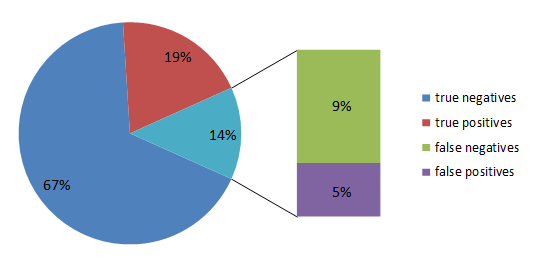
\includegraphics[scale=.8,angle=0]{images/Experiment01.png}
		\vspace*{-1mm}
		\caption{\textbf{RDF-Doctor evaluation with Turtle Test Suite \cite{TurtleTests:Online}.} Each file in \cite{TurtleTests:Online} was classified as having a syntax error or not. Then, the final results were grouped into 4 categories: true positives (files with syntax errors  correctly identified); false positives (files without syntax errors  incorrectly identified); false negatives (files with syntax errors  incorrectly rejected); true negatives (files without syntax errors  correctly rejected).}
		\label{Fig:Experiment01}
\end{center}
\end{figure}

 Table \ref{tab:detection} evaluates RDF-Doctor with the referred input. This table features a classification of error types which helps to group those types into categories to ease the research work. Details about types of errors can be found in Appendix~\ref{ch:synErrCategories}. In order to evaluate the automatic error correction feature of RDF-Doctor. The input of this experiment was used. The result shows that 5 types of errors can be faultlessly corrected. They are listed in Table \ref{tab:detection} with Serial Numbers (SN): 4, 39, 53, 54, and 55 and the type of syntax error that can be automatically corrected are: 1) using of `A' as a predicate instead of `a'; 2) missing a colon in prefix or base declarations; 3) missing  a dot at the end of a triple; 4) adding more than one dot a the triple end; and 5) ending a triple with a semi-colon instead of a dot, correspondingly.       

\section{Experiment II}

In the following, we provide details about the second experiment where RDF-Doctor is validated through a synthetic experiment. 

\subsection{Objective}
The objective was to simulate a real world scenario where an ontology engineer develops an ontology for a particular domain using a plain text editor.
During work, which commonly lasts eight hours, the engineer may perform several changes to the ontology, while saving it during each hour.
While doing that, the engineer may introduce a number of syntactic errors, which he has to identify and correct before being able to share his contribution with other team members.
%To get rid of the generated bias, this experiment uses both Poisson distribution and uniform random number generation methods. It also assumes a naive user editing an RDF input data, found in an environment similar to the one in Figure \ref{Fig:Motivation} and he is mistakenly generating some  syntax errors. Then, the inserted syntax errors evaluate the quality of RDF-doctor.

\begin{figure}[ht]
	\begin{center}
		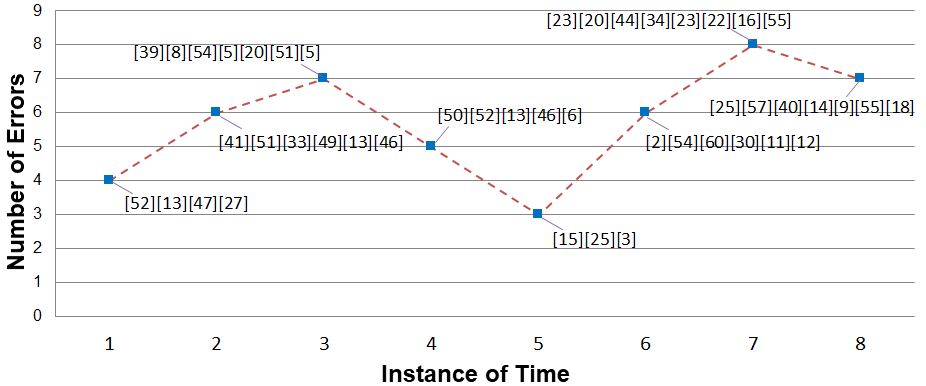
\includegraphics[width=1\linewidth,angle=0]{images/Experiment02-01.png}
		\vspace*{-3mm}
		\caption{\textbf{Distribution of syntax errors.} The Number and types of syntax errors between brackets for an interval of eight instances of time. 
		A Poisson Distribution with the parameter $\lambda$ = 5 models an average of five syntax errors per instance of time. 
		Each instance of time shows value of $\lambda$, assuming the ontology engineer can generate between 1 to 10 syntax errors per instance of time. 
		Also, a Uniform Distribution generates random numbers in the interval between 1 and 61, to select the error type as listed in Appendix~\ref{ch:synErrCategories}. 
		For example, at the 5\textsuperscript{th} instance of time, three error types are introduced, i.e., [3,15,25].} 
		\label{Fig:experiment2}
	\end{center}
\end{figure}

\subsection{Procedure}

In this experiment, we assume that while the ontology engineer contributing to the DBpedia ontology performs several modifications, e.g. insert, edit or delete during a period of eight instances of time, i.e., each hour. 
The Poisson and Uniform Distribution are used to simulate the number and the type of errors occurred in each instance of time, respectively.
The average number of syntax errors per instance of time is represented by $\lambda$ parameter. 
For example, $\lambda$ = 5, means that five syntax errors are occurred per hour on average.  
%As an input for a Poisson distribution, 10 syntax errors per instance of time was supplied. 
The Uniform Distribution is used to randomly select the error types from a comprehensive list of errors as given in Appendix~\ref{ch:synErrCategories}.
%Hence, for each instance of time we calculate value of $\lambda$, then the output value drives how many number of syntax errors are entitled for that instance of time.
%Next, Those syntax errors are arbitrarily selected from the type of errors range [1-61], drawn by rows of Table . 
Moreover, the exact location for injecting syntax errors within the RDF file is realized using the Uniform Distribution where a random line number is generated.
The error is successfully applied if the randomly selected location is appropriate for the error type; Otherwise, one of the lines for its neighborhood is selected. 
If the error is related to the header (the top of the file where directives are normally located), the injection is applied into a region of directives.  

	\begin{figure}[ht]
	\begin{center}
		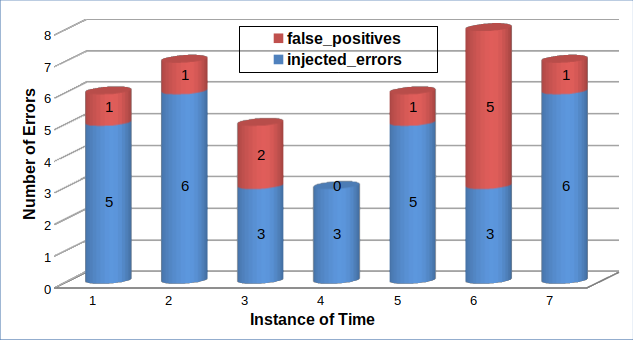
\includegraphics[scale=0.9,angle=0]{images/Experiment02-02.png}
				\vspace*{-4mm}
		\caption{\textbf{Error detection when syntax errors are randomly distributed.} 
		For each instance of time, a number of errors which are detected or not detected by RDF-Doctor are shown.
		%"detected", and those one which were undetected and unrecognized by RDF-Doctor, referred as "undetected".
		} 
		\label{Fig:Experiment02-02}
	\end{center}
\end{figure}



\subsection{Result and Discussion}

Experimental results illustrated in Figure \ref{Fig:Experiment02-02} show that RDF-Doctor in a majority of the cases is able to correctly recognize syntax errors. 
More specifically, in half of the instances time, apart from one syntax error not recognized, all of them are identified.
In time instance number 5, all errors are detected.
However, there are some instances of time where more than one error is not recognized, such as time instance number 7 with five undetected syntax errors.
The reason behind a high number of undetected syntax errors is that most of the unrecognized syntax errors by RDF-Doctor are involved in the injected errors during that time instance. The proper solution for such an issue can be achieved by improving the recognition ability of RDF-Doctor of all kinds of syntax errors.


Figure \ref{Fig:Experiment02-03} illustrates a comparison of the number of the injected errors versus the number of false positives of this experiment. 
As we can observe, the average number of false positives is high which may result due the probability of the existence of one or more unrecognized syntax errors which are coming from the libraries of the ANTLR framework. 
One possible solution for this is by to optimize RDF-Doctor by developing an additional layer to internally handle these type of errors aside from  the error production rules for a particular grammar.

%rest of the times instances show zero or few errors, except the time instance number 6\textsuperscript{th}, , this can be due to fall most of the unrecognized syntax errors in this time instance since the insertion of the syntax errors was done randomly.  

\begin{figure}[ht]
	\begin{center}
		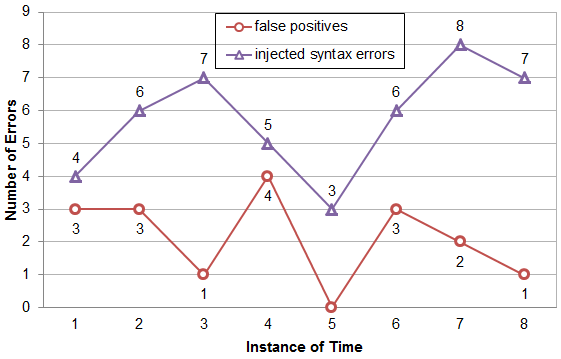
\includegraphics[width=0.9\linewidth,angle=0]{images/Experiment02-03.png}
				\vspace*{-4mm}

		\caption{\textbf{Result of false positives during RDF-Doctor validating with randomly distributed syntax errors.}
		For each time instance, when a number of syntax errors are randomly inserted, it may result in false positives since one of the unrecognized syntax errors can be in-between the inserted ones.} 
		\label{Fig:Experiment02-03}
	\end{center}
\end{figure}
 


\section{Experiment III}

This experiment evaluates the behaviour and the performance RDF-Doctor by changing the number of syntax errors and the size of ontologies. 

\subsection{Objective}
The objective was to check the effect on the behaviour and the performance of our approach whenever the number of errors increases.
Furthermore, we evaluated the performance of RDF-Doctor when the size of the ontologies is changed, to simulate real world scenarios where ontologies continue growing over the time.

%We are studying the effect of growing of number of syntax errors, as well as, the size of ontologies when it is changed. 


\subsection{Procedure}

We used two types of ontologies; small and medium sized. 
The Friend of a Friend Vocabulary (FOAF)~\footnote{\url{http://www.foaf-project.org/}} is used as a small ontology with a total number of 631 triples. 
As a medium sized ontology, we used DBpedia~\footnote{\url{https://wiki.dbpedia.org/develop/datasets/dbpedia-version-2016-10}} version 2016-10 with a total number of 30,790 triples. 
In both ontologies three different numbers of syntax errors were introduced i.e., 10, 30, 61. These syntax errors were randomly injected using  the same way as in the previous experiment where the Uniform Distribution is utilized.
Additionally, to avoid any impact on the current overload of the processor during the execution time, we ran our experiment five times for each case and calculated the average processing time.

 \begin{figure}[ht]
\begin{center}
		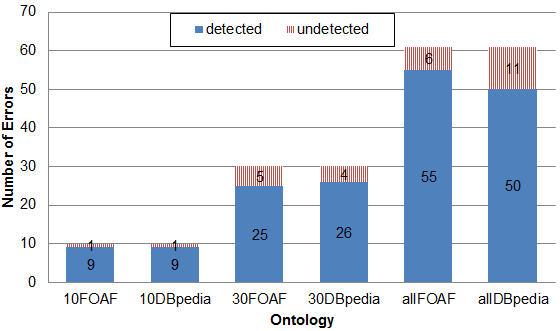
\includegraphics[scale=0.9,angle=0]{images/Experiment03-01.png}
		\vspace*{-4mm}
		\caption{\textbf{Impact of number of errors and the size on error detection.} 
		FOAF and DBpedia ontologies are used to evaluate RDF-Doctor, 10foaf, 30foaf, allfoaf are datasets of FOAF ontology, including with 10, 30, 61 random syntax errors, respectively; same is applicable for DBpedia. Detected errors are the errors which were properly identified by RDF-Doctor matched error messages  released, while undetected errors are those which were not correctly recognized.}
		\label{Fig:Experiment03-01}
\end{center}
\end{figure}
\subsection{Result and Discussion}
Figure \ref{Fig:Experiment03-01} illustrates the performance of the number of errors and the ontology size. 
After introducing 10 syntax errors, 9 out of 10 were detected and one was not detected for both FOAF and DBpedia ontologies. 
In the second case, 25 out of 30 injected errors were detected in FOAF, and 26 out of 30 injected errors in DBpedia were detected. 
Finally, of 61 injected errors, 6 in FOAF and 11 DBpedia were not detected.
In all the cases, for each error that was detected, an expressive message was given to help users to resolve them. 




\begin{figure}[ht]
\begin{center}
		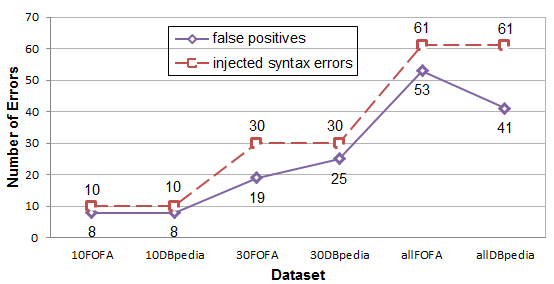
\includegraphics[scale=0.9,angle=0]{images/Experiment03-02.png}
		\vspace*{-4mm}
		\caption{\textbf{Result of false positives when number of errors and ontology size are increased.} Unrecognized errors may generate more false positive errors than actual errors. 
		%and when the number of errors increase, the false positives are comparably increased.
		}
   \label{Fig:Experiment03-02}
\end{center}
\end{figure}
Another essential point is the number of false positives as shown in Figure \ref{Fig:Experiment03-02}. 
It can be seen that the false positives are incremented while raising the number of syntax errors.
This comes as a consequence of increasing the number of unrecognized syntax errors, forcing the parser to try to recover from such errors by adding or removing some tokens, which in turn produces an increased number false positives.   


The performance of RDF-Doctor is presented in Figure \ref{Fig:Experiment03-03}. 
It summarizes the impact of both the number of errors and the ontology size on the RDF-Doctor performance.
As we can observe, the numbers of errors has no influence on the performance, i.e., the processing time is similar in either FOAF or DBpedia while changing number of errors. 
On the other hand, the size of ontologies has a high impact on the overall performance, i.e, processing DBpedia consumes about 29000ms in average; whereas, FOAF is parsed in about 2000ms. In conclusion, approximately more than 90\% of injected syntax errors were detected, as shown in Figure~\ref{Fig:Experiment03-01}. 
%Also, number of false positives can be improved if RDF-Doctor recognized those undetected errors by either do more laboratory works to match those patterns or may with the new versions of ANTLR library.  
%talk about the correction of errors #numbers 

\begin{figure}[ht]
\begin{center}
		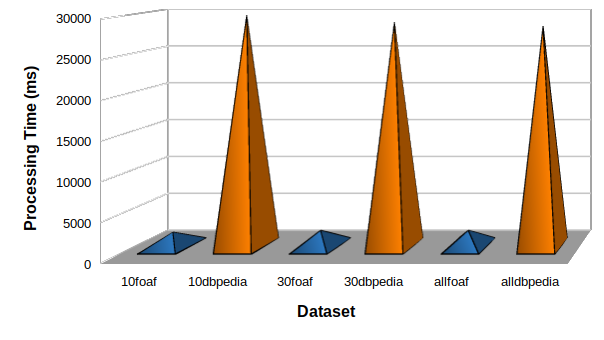
\includegraphics[scale=0.9,angle=0]{images/Experiment03-03.png}
		\vspace*{-4mm}
		\caption{\textbf{Performance evaluation when a number of errors and ontology size is changed, individually.} 
		Performance is calculated with required processing time, i.e., in miliseconds (ms) in both cases: 1) 10, 30, and 61 injected syntax errors; 2) FOAF ontology with 631 triples and DBpedia ontology, with 30,790 triples.}
\label{Fig:Experiment03-03}

\end{center}
\end{figure}
